\documentclass[a4paper,10pt,onecolumn]{article}


\usepackage[margin=2cm]{geometry}
\usepackage[ruled,vlined]{algorithm2e}
\usepackage{amsmath}
\usepackage{dsfont}
%\usepackage{xfrac}
\usepackage[dvips]{graphicx}

\graphicspath{{./../Figures/}}
\DeclareGraphicsExtensions{.eps}

\begin{document}

% Text related command shortcuts

\newcommand{\bi}[1]{\textbf{\textit{#1}}}

% Math related command shortcuts

\newcommand{\mbi}[1]{\mathbf{\mathit{#1}}}
\newcommand{\mbf}[1]{\mathbf{#1}}

\newcommand{\mscrmxy}[2]{{#1}_{\mathrm{#2}}}
\newcommand{\msclxy}[2]{{#1}_{\mathit{#2}}}
\newcommand{\msclxyz}[3]{{#1}_{\mathit{#2},\mathit{#3}}}

\newcommand{\mvecxy}[2]{\mathbf{#1}_{\mathit{#2}}}
\newcommand{\mvecxyz}[3]{\mathbf{#1}_{\mathit{#2},\mathit{#3}}}

\newcommand{\me}[1]{\(#1\)}
\newcommand{\mrm}[1]{\mathrm{#1}}
\newcommand{\mc}[1]{\mathcal{#1}}
\newcommand{\mtext}[1]{\mathit{#1}}

\newcommand{\mxu}[2]{\mathbf{#1}^{\mathit{#2}}}
\newcommand{\mxl}[2]{\mathbf{#1}_{\mathit{#2}}}
\newcommand{\mxul}[3]{\mathbf{#1}^{\mathit{#2}}_{\mathit{#3}}}

\newcommand{\inm}{\, \in \,}
\newcommand{\fall}{\, \forall \,}
\newcommand{\bs}{\: \backslash \:}
\newcommand{\card}[1]{| \, #1 \, |}
\newcommand{\norm}[2]{\|\, #1 \,\|_{#2}}
\newcommand{\gnorm}[1]{\|\, #1 \,\|}
\newcommand{\sset}{\, \subset \,}

\newcommand{\inmt}[1]{\( \mathit{#1} \)}
\newcommand{\mcxy}[2]{\mathcal{#1}_{\mathit{#2}}}

\newcommand{\argmax}{\operatorname*{\arg\,max}}

% Math environment command shortcuts

\newenvironment{ceq}{\begin{center}\begin{equation}}{\end{equation}\end{center}}
\newenvironment{cneq}{\begin{center}\begin{equation*}}{\end{equation*}\end{center}}

\newenvironment{ceqn}{\begin{center}\begin{eqnarray}}{\end{eqnarray}\end{center}}
\newenvironment{cneqn}{\begin{center}\begin{eqnarray*}}{\end{eqnarray*}\end{center}}


\section{Introduction}

\section{System Model}


The system model considers \me{\mscrmxy{N}{B}} BSs, each has \me{\mscrmxy{N}{T}} transmit antennas and \me{K} users with a single receive antenna. The set \me{\mcxy{U}{b}} denotes the set of users linked to BS \me{b} where \me{b \in \{1,2,\dotsc,\mscrmxy{N}{B}\}}. The set \me{\mc{U}} given by \me{\mcxy{U}{b} \sset \mc{U}} represents the total users in the system as represented by \me{\card{\mc{U}} = K}. The set \me{\mcxy{B}{k} \sset \mc{B} = \{1,2,\dotsc,\mscrmxy{N}{B}\}} represents the set of BSs transmitting for the user \me{k}. The cardinality of the set \me{ \card{\mcxy{B}{k}} \geq 1} represents the coordinated transmission from more than one BS in the system. The users are statically assigned to a BS in the single BS transmission scenario based on the pathloss measures. The received signal \me{\msclxy{y}{k}} of the user \me{k} consisting of both inter cell and intra cell interference is given by
\begin{eqnarray}
\msclxy{y}{k} = \underbrace{\sum_{\mtext{b} \inm \mcxy{B}{k}} \mvecxyz{h}{b}{k} \mvecxyz{x}{b}{k}}_{\mathclap{\text{desired term}}} \quad + \quad \overbrace{\sum_{\mtext{b} \inm \mcxy{B}{k}} \mvecxyz{h}{b}{k} \sum_{\mathclap{\mtext{i} \inm \mcxy{U}{b} \bs \mtext{k}}} \mvecxyz{x}{b}{i}}^{\mathclap{\text{intra cell interference terms}}} \quad + \quad \overbrace{\sum_{\mathclap{\mtext{c} \inm \mc{B} \bs \mcxy{B}{k}}} \mvecxyz{h}{c}{k} \sum_{\mtext{j} \inm \mcxy{U}{c}} \mvecxyz{x}{c}{j}}^{\mathclap{\text{inter cell interference terms}}} \quad + \quad \msclxy{n}{k}
\label{sm-e1}
\end{eqnarray}

where the vector \me{\mvecxyz{x}{b}{k} \inm \mathds{C}^{\mscrmxy{N}{T}}} represents the transmitted symbol from the BS \inmt{b} to user \inmt{k}, \me{\msclxy{n}{k} \sim \mc{CN}(0,\mtext{N}_0)}, and \me{\mvecxyz{h}{b}{k} \inm \mathds{C}^{1 \times \mscrmxy{N}{T}}} denotes the channel (including pathloss) between the BS \inmt{b} to the user \inmt{k}.

The transmitted symbol \me{\mvecxyz{x}{b}{k}} for the user \inmt{k} from BS \inmt{b} is given by \me{\mvecxyz{x}{b}{k} = \mvecxyz{m}{b}{k} \, \msclxy{d}{k}} where \me{\mvecxyz{m}{b}{k}} is the precoder used by the BS \inmt{b} for user \inmt{k} and \me{\msclxy{d}{k}} denotes the data meant for user \inmt{k} with \me{\mbf{E} [\, \card{d}^2 ] = 1}. The total power used by the transmitter is given by
\begin{equation}
\sum_{k \inm \mcxy{U}{b}} \mrm{Tr} \left ( \mvecxyz{x}{b}{k} \, \mvecxyz{x}{b}{k}^{\mrm{H}} \right ) \leq \mrm{P}_{t}
\label{sm-e2}
\end{equation}

The precoding scheme is based on weighted minimum mean squared error (W-MMSE) scheme discussed in \cite{wmmse_shi} or by combined zero-forcing (CZF) scheme by stacking the channel of users in the transmission set of all BSs in \me{\mc{B}} as discussed in \cite{spencer2004zero}. Once precoders are defined, power allocation is performed over precoders designed by CZF scheme to either maximize the sum capacity or to minimize the expected queue size. W-MMSE based precoding scheme is also analyzed in this paper to bring out the performance comparison. W-MMSE scheme provides joint design of precoder and power allocation for each users in the network.

Scheduling schemes are compared with the well established schemes discussed in \cite{sus2006zfbf,zhang2007user} which aims at selecting least correlated users for the transmission set for MU-MIMO. The selection process is performed in an iterative manner by selecting the first user based on the channel norm.
\begin{eqnarray}
\mbf{N} &=& \mbf{I} - \mbf{U} ( \, \mbf{U}^\mrm{H} \mbf{U} \, )^{-1} \mbf{U}^\mrm{H} \label{sm-e3} \\
\mbf{U} &=& \matscont{\mvecxyz{h}{b}{x}^\mrm{T} \; \mvecxyz{h}{b}{y}^\mrm{T}} \fall x,y \inm \mc{S}_b \text{ where } b \inm \mc{B} \nonumber
\end{eqnarray}
The successive users are chosen by selecting the user with the highest projection gain over the null space formed by the channel vectors of the already chosen users at BS \me{b} as given by
\begin{equation}
j = \argmax_i \gnorm{\mbf{N}^\mrm{H} \mvecxyz{h}{b}{i}^\mrm{T}} \, \fall i \inm \mc{U}_b.
\end{equation}
The user \me{j} is then selected as the next user in the transmission set and the process is repeated until the transmission user set \me{\card{\mc{S}_b} = N_\mrm{T}}. The selection schemes discussed in \cite{jin2010novel,ko2012determinant} performs similar to the one discussed earlier but with different interpretation which is based on maximizing the volume formed by the user channel vectors.

The scheduling schemes discussed are not limited to single receive antenna; it can be extended for multi antenna by treating each spatial streams as virtual users using singular value decomposition (SVD) over the channel matrix of users in \me{\mc{U}}. The precoder design using W-MMSE scheme is straight forward with the transmission user set selected based on scheduling schemes as it optimizes both transmit and receive beamformers jointly. The zero-forcing precoding is performed in an iterative manner by fixing the receive beamformers using MMSE receivers as discussed in \cite{antti_user_selection}.


\section{Single BS User Scheduling} \label{sbus}

The user selection scheme for MU-MIMO transmission performs better when the user \inmt{k \in \mcxy{U}{b}} channels are uncorrelated. The uncorrelated channel constraint helps in decoupling the users data streams with the help of precoders thereby providing interference free transmission. The selection of users with two different objective is studied in this section namely, capacity achieving and fairness based queue size reduction. The channel represented by \me{\mvecxyz{h}{b}{k}} is given by \me{\mvecxy{h}{k}} by dropping the subscript corresponds to BS \me{b = 1}.

\subsection{Max-Throughput based User Scheduling} \label{mtbus}

The selection methods with the objective of maximizing the overall throughput is considered in this section. The algorithms mentioned here are classified based on the performance and complexity. The complexity involved is lowered by reducing the operations involved in calculating the metric used for comparison.

\subsubsection{Eigen vector based User Selection}


The main objective of capacity achieving MU-MIMO transmission is to select the users whose channel vectors are uncorrelated. Uncorrelated channels can be de-coupled easily to facilitate interference free transmission with the use of precoders. The measure of uncorrelated vectors can be obtained by finding determinant of the inner product of stacked  channel vectors. The capacity achieving user selection is carried out by forming a matrix \me{\mbf{M}} of size \me{K \times K} where \me{K = \card{\mcxy{U}{1}} = \card{\mc{U}}} which describes the number of users in a given BS.

The matrix \me{\mbf{M}} is populated with the metric which holds information about the co-existence measure between the users corresponding to the \me{i^{\mrm{th}}} row and \me{j^{\mrm{th}}} column. The metric also includes the channel vectors of users already selected for transmission at a given scheduling resource. The metric used at each element of the matrix \me{\mbf{M}} is given by
\begin{eqnarray}
\mbf{T} &=& \left [\,\mbf{T}_\mrm{o} \; \mvecxy{h}{i}^\mrm{T} \; \mvecxy{h}{j}^\mrm{T} \, \right ] \\
\msclxyz{M}{i}{j} &=& \det{\left ( \, \mbf{T}^{\mrm{H}} \; \mbf{T} \, \right )} \label{mca1-e1:2}
\label{mca1-e1}
\end{eqnarray}
where \me{\mbf{T}_\mrm{o}} denotes the stacked channel vectors of users belonging to the transmission set \me{\mc{S}, \, \card{\mc{S}} \leq N_\mrm{T}} at a given scheduling instant. The set \me{\mc{S}} is initialized with \me{\emptyset} and users are included in the set incrementally. Once the matrix \me{\mbf{M}} is populated, a user is selected based on the method followed in analytic hierarchy process (AHP) as in \cite{saaty2008decision}. The matrix \me{\mbf{M} \succeq 0}, Eigen value decomposition (EVD) decomposes the matrix into \me{\mbf{P} \, \mbf{D} \, \mbf{P}^\mrm{T}} where \me{\mbf{P}} is a unitary matrix consists of Eigen vectors of \me{\mbf{M}} and \me{\mbf{D}} is a diagonal matrix having Eigen values on its diagonal entries.

Let \me{\msclxyz{D}{k}{k}} represents the maximum Eigen value at \me{k^{\mrm{th}}} index and the corresponding Eigen vector is given by \me{\mvecxy{p}{k}}. Since each entry \me{\msclxyz{p}{i}{k} \fall i \inm \{1,2,\dotsc,K \}} has unequal gains which corresponds to the significance of the entry in achieving the corresponding Eigen gain, user \me{i} is selected with
\begin{eqnarray}
i &=& \argmax_{\mathrm{i}} \norm{\msclxyz{p}{i}{k}}{2} \label{mca1-e2:1} \\
\mc{S} &=& \left \lbrace \, \mc{S} \, \cup \, i \, \right \rbrace.
\label{mca1-e2}
\end{eqnarray}

Selection is carried out in an iterative manner with the stopping criterion given by \me{\card{\mc{S}} = N_\mrm{T}} as detailed in Algorithm. \ref{mca1-a1}. Precoding is performed over the channels of the users in \me{\mc{S}} which forms the transmission set. Precoding is either zero-forcing (ZF) with water-filling power allocation (WF-PA) as in \cite{tse2005fundamentals} or weighted sum rate maximization using weighted minimum mean squared error (W-MMSE) as given in \cite{wmmse_shi} with the power constraint as given in \eqref{sm-e2}.

\begin{algorithm}
 \SetAlgoLined
 \DontPrintSemicolon
 \KwIn{\me{\mvecxy{h}{k} \fall k \inm \mc{U} }}
 \KwData{\me{\mc{S} = \emptyset, \, \mbf{M}, \, \mbf{T}_\mrm{o} = [\,]}}
 \While{\me{\card{S} \leq N_\mrm{T}}}{
 \ForEach{\me{ \msclxyz{M}{i}{j}, \, \mrm{where} \, i,j \inm \{1,2,\dotsc,K\}}}{
 formulate \me{\msclxyz{M}{i}{j}} using \eqref{mca1-e1:2} \;
 }
 perform EVD as \me{\mbf{M} = \mbf{P} \, \mbf{D} \, \mbf{P}^\mrm{T}} \;
 select user \me{i} using \eqref{mca1-e2:1} \;
 \me{\mc{S} = \{ \, \mc{S} \cup i \, \}}, \me{\mbf{T}_{\mrm{o}} = \left [\, \mbf{T}_{\mrm{o}} \, \mvecxy{h}{i} \, \right ]} \;
 }
 \caption{Eigen Vector based User Selection}
 \label{mca1-a1}
\end{algorithm}


\subsubsection{Selection based on Reduced Null Space Gain}


The objective of capacity achieving user selection and the complexity involved in implementing the same is considered. The proposed method provides and alternative way to achieve the null space calculations involved in the selection procedure. User selection based on QR based decomposition requires null space formulation in order to find the orthogonal subspace for the given vector channel were discussed in \cite{traniterative,zhang2007user,sun2009eigenmode}.

The user channels are projected on to the null space of the existing users channel vectors in \me{\mc{S}} where \me{\mc{S}} represents the users selected for the current scheduling instant. The null space is approximated by the product of the vertical projection distance from the given channel vector to the existing users channel vectors in \me{\mc{S}}. The channel vector \me{\mvecxy{h}{i} \fall i \inm \mc{U}} is projected on to the matrix \me{\mbf{U}} formed by stacking the normalized channel vectors of the users in \me{\mc{S}}.
\begin{equation}
\mbf{U} = \left [ \, \frac{\mvecxy{h}{i}^\mrm{T}}{\gnorm{\mvecxy{h}{i}}}, \dotsc, \frac{\mvecxy{h}{j}^\mrm{T}}{\gnorm{\mvecxy{h}{j}}} \, \right ], \; \fall i,j \inm \mc{S}
\label{mca2-e1}
\end{equation}
In order to find the vertical projection distance, channel vector of the users in \me{\mc{U}} is projected on \me{\mbf{U}} is  denoted by \me{\mbf{g}}. The vector \me{\mbf{g}} contains the projection gains of the given channel vector onto the normalized channel of the users in \me{\mc{S}} as
\begin{equation}
\mbf{g} = \mbf{U}^\mrm{T} \mvecxy{h}{i}, \fall i \inm \mc{U}
\label{mca2-e2}
\end{equation}
The vertical projection distance is given by subtracting the norm of channel vector from the projection metric \me{\mbf{g}}. The null space projection is then obtained by multiplying the vertical projection distance from all the unit vectors from the given channel vector as
\begin{equation}
\msclxy{m}{i} = \prod^{\card{\mc{S}}}_{l = 1} \left ( \, \gnorm{\mvecxy{h}{i}} - \card{g_l} \, \right ), \fall i \inm \mc{U}
\label{mca2-e3}
\end{equation}
where \me{g_l} represents \me{l^\mrm{th}} element in \me{\mbf{g}} and \me{\msclxy{m}{i}} denotes the null space projection of user \me{i} on to the existing user set \me{\mc{S}}.

The product measures the gain achieved by projecting the vector \me{\mvecxy{h}{i}} over the null space of the vectors formed by the channel vectors of users in the set \me{\mc{S}}. The product yields `\me{0}' when the vector \me{\mvecxy{h}{i}} is in the direction of the unit channel vectors in \me{\mbf{U}}. The product will not provide `\me{0}' when it is collinear with any two vectors in \me{\mbf{U}} as given by null space. Even though this method provides an approximation for null space, performance achieved by this scheme is closer to that of the selection scheme achieved by null space based projections discussed in \cite{sus2006zfbf,icsps2010}. The pseudo code is briefed in the Algorithm. \ref{mca2-a1}.

\begin{algorithm}
 \SetAlgoLined
 \DontPrintSemicolon
 \KwIn{\me{\mvecxy{h}{k} \fall k \inm \mc{U} }}
 \KwData{\me{\mc{S} = \emptyset, \, \mbf{U} = [\,]}}
 \While{\me{\card{S} \leq N_\mrm{T}}}{
 \ForEach{\me{ i \inm \{1,2,\dotsc,K\}}}{
 formulate \me{\mbf{U}} using \eqref{mca2-e1} \;
 calculate \me{\msclxy{m}{i}} using \eqref{mca2-e2}, \eqref{mca2-e3} \;
 }
 select user \me{\displaystyle k = \argmax_i \: \msclxy{m}{i}} \;
 \me{\mc{S} = \{ \, \mc{S} \cup k \, \}} \;
 }
 \caption{Selection based on Reduced Null Space Gain}
 \label{mca2-a1}
\end{algorithm}

\subsection{Queue based User Scheduling} \label{qbus}

In this section, we discuss the selection schemes which considers the queue backlogs of each user and aims at minimizing it for each users in the set \me{\mc{U}}. Even though the users are selected based on the objective of minimizing the queues, power allocation based on water-filling (WF-PA) for zero-forcing (ZF) precoders has the objective of maximizing the sum capacity. The WF-PA scheme is replaced with the queue based power allocation scheme which uses queue weighted sum rate maximization objective (QW-PA).

The W-MMSE based precoding scheme is also analyzed in this section for the precoder design with the expected queue minimizing objective. The following section discusses two selection schemes with the objective of reducing the queues namely weighted user selection and percentile proportional fair scheduling scheme.

\subsubsection{Queue weighted User scheduling} \label{weighted-queue-sched}


User selection which has the objective of reducing the expected queue of each user select users with higher queue backlogs. The selection strategy based on queue and the channel condition is discussed extensively in \cite{neely2012stability}. The queue based selection based on Lyapunov drift reduction along with power reduction is also discussed. The performance of those schemes are well suited for single user MIMO (SU-MIMO) where the entire spatial dimension is allotted for a single user.

In case of MU-MIMO, the users sharing spatial dimension will share the power and moreover interfere with each other unless precoder decouples the transmitted data. In order to decouple the transmitted data, the channel of the users in \me{\mc{S}} should be uncorrelated spatially. Once precoders are designed, power allocation for each users is performed based on queues and the channel condition in order to minimize the expected queue length for each users.

Let \me{\mbf{Q}_i(n)} represents the backlog packets at \me{n^\mrm{th}} instant and \me{\mbf{b}_i(n)} represents the transmission bits at \me{n^\mrm{th}} instant for \me{i^\mrm{th}} user. The Lyapunov formulation is based on minimizing the queue variation at \me{n} and \me{n + 1} instant. The queue update at \me{n+1} is given by
\begin{equation}
\mbf{Q}(n+1) = \min \setcont{\mbf{Q}(n) - \mbf{b}(n),0} + \lambda(n)
\end{equation}
and the Lyapunov drift minimization is given by
\begin{eqnarray}
L(\mbf{Q}(n + 1)) - L(\mbf{Q}(n)) &=& \mbf{Q}(n + 1)^2 - \mbf{Q}(n)^2 \\
&=& \matscont{\min \setcont{\mbf{Q}(n) - \mbf{b}(n),0} + \lambda(n)}^2 - \mbf{Q}(n)^2
\label{qba1-e0}
\end{eqnarray}
where \eqref{qba1-e0} is optimized to minimize the Lyapunov drift as discussed in \cite{neely2010stochastic}.

Upon reducing the formulation in \eqref{qba1-e0} with the minimizing objective, the drift minimizing user scheduling for the set \me{\mc{S}} is given by
\begin{eqnarray}
&\displaystyle \max_{\mc{S} \inm \mc{U}} \, \sum_{i \inm \mc{S}}\mbf{Q}_i(n) \, \mbf{b}_i(n) \\
&\displaystyle \mrm{subject \: to,} \quad \card{\mc{S}} \leq N_\mrm{T}.
\label{qba1-e1}
\end{eqnarray}
The above problem is difficult to solve due to the constraint \eqref{qba1-e1} which casts it as a combinatorial search problem. The suboptimal solution is proposed by considering user selection in an incremental manner as seen in Sect. \ref{mtbus}. Since \me{\mbf{b}(n)} is given by \me{ \textstyle \log \left \lbrace 1 + \frac{\gnorm{\mvecxy{h}{i}}^2}{N_\mrm{0}} \right \rbrace } at \me{n^\mrm{th}} instant, the optimization function for the user \me{i} is given by
\begin{eqnarray}
&\displaystyle \max_{\fall i \inm \mc{U}} \, \mbf{Q}_i \, \log \left \lbrace 1 + \frac{P_\mrm{i} \; \gnorm{\mvecxy{h}{i}}^2}{N_\mrm{0}} \right \rbrace \\
&\displaystyle \max_{\fall i \inm \mc{U}} \, \mbf{Q}_i \, \left [ \; 2 \, \log \left \lbrace P_\mrm{i} \; \gnorm{\mvecxy{h}{i}} \right \rbrace - \log \left \lbrace N_\mrm{0} \right \rbrace \; \right ]
\label{qba1-e2}
\end{eqnarray}
where \eqref{qba1-e2} is based on high-SNR approximation. Since \me{N_\mrm{0}} is constant and can be dropped, the approximated objective is given by \me{\max_i \mbf{Q}_i \: \mvecxy{h}{i}} where \me{\log \{x \} \approx x}. The sharing of total transmission power among \me{\mc{S}} is not known during user selection, the optimization objective includes only the channel norm with path loss in the final formulation.

The queue weighted user selection is performed as briefed in \cite{sus2006zfbf,sun2009eigenmode} with queue weighted channel vectors. This scheduling provides queue stability and reduces the expected queue size for each user \cite{neely2012stability}. If precoder is based on ZF, power allocation needs to be performed with the objective of maximizing the sum rate with queue as weights to achieve the above discussed optimization objective.



\subsubsection{Percentile proportional fair scheduling}


The queue stability can be achieved by scheduling users based on their respective queue backlogs and their instantaneous channel state information. Proportional fair scheduling achieves this objective by weighing the rate fairness metric \me{\displaystyle {\mbf{r}_i}/{\mbf{R}_i}} with the queue backlogs \me{\mbf{Q}_i}, where \me{\mbf{r}_i, \: \mbf{R}_i} represents the instantaneous and average rate of user \me{i}. The variants of proportional fair scheduling for multi carrier transmissions with different objectives were discussed in \cite{adaptation_crosslayer}.

The fairness objective discussed in \cite{adaptation_crosslayer} perform well for single antenna transmission where the users are separated orthogonally by time or frequency. In case of MU-MIMO transmission, the performance are limited due to the co-channel interference when users are multiplexed in the spatial dimension. In order to provide scheduling fairness and interference free transmission, users selected based on fairness metric should also have uncorrelated channel vectors for efficient decoupling of transmission using precoders.

The proposed scheme achieves the above mentioned objective by considering two level user selection strategy. In the first level, the transmission set \me{\mc{S}} is selected based on the sorted proportional fair metric with queue as the priority factor \me{f_i = {\mbf{r}_i \mbf{Q}_i} / {\mbf{R}_i}} where \me{f_i} is the \me{i^\mrm{th}} user fairness metric of the vector \me{\mbf{f}}. Let \me{\mbf{f}_{\pi}} represents the sorted fairness metric in the descending order. The user set \me{\mc{F}_\pi} is populated with \me{x} percentile users based on sorted fairness metric \me{\mbf{f}_\pi} as
\begin{equation}
\mc{F}_\pi = \left \lbrace \: i \mid \arg_i \: \msclxyz{f}{\pi}{i} \geq \msclxyz{f}{\pi}{x}, \fall i \inm \mc{U} \: \right \rbrace
\end{equation}
where \me{x = 50} corresponds to \me{50 \% \: \text{ile}} user selection.

The second level of user selection is performed over the subset \me{\mc{F}_\pi} which has users with better fairness metric over \me{\mc{F}^c_\pi = \mc{U} \bs \mc{F}_\pi}. The user selection is carried out based on queue weighted user scheduling discussed in Sect. \ref{weighted-queue-sched} over the reduced user set \me{\mc{F}_\pi}. The selection procedure achieves fairness objective from the initial user selection and the spatial separation based on the weighted queue user scheduling scheme.


\section{Multi BS User Scheduling}

The selection of users to maximize the system throughput with multiple BS is considered here. The scheduling schemes based on the user set over which the selection is carried out for multi-BS scenario is addressed in this section.

\subsection{Static User Scheduling} \label{sus}


This section discusses the user selection strategy performed over the set \me{\mc{U}_b \sset \mc{U}} which represents the users linked to BS \me{b}. The selection performed over the associated user set \me{\mc{U}_b, \fall b \inm \mc{B}} provides the transmission set \me{\mc{S}_b} of BS \me{b} which needs to be signalled to all BSs in the set \me{\{ \mc{B} \bs b \}}. The selection is carried out in an iterative manner with the limited signaling between the cooperating BSs to maximize the overall sum throughput.

In multi-BS scenario, the available spatial dimension \me{N_\mrm{T}} is shared between the transmission of information to the desired cell users and minimizing the interference created to the neighboring cells. This is performed by sharing the available spatial freedom \me{N_\mrm{T}} over the cooperating BSs in \me{\mc{B}} by dividing the spatial dimension over \me{\card{\mc{B}}} as given by \me{\left \lfloor \frac{N_\mrm{T}}{N_\mrm{B}} \right \rfloor} with the assumption \me{N_\mrm{T} \geq N_\mrm{B}}. In order to discuss the scheme, let \me{\mc{S}^{i}_{\cup} = \{ \mc{S}_1 \cup \mc{S}_2 \cup \dotso \cup \mc{S}_{N_\mrm{B}} \}} represents the transmission user set of the network at \me{i^\mrm{th}} iteration and 
\me{\mc{S}^i_{\cup,b} = \{ \mc{S}^i_{\cup} \bs \mc{S}_b \} } represents the transmission user set excluding BS \me{b}.

To begin with, initialize \me{\mc{S}_j \fall j \inm \mc{B}} and \me{\mc{S}^i_{\cup}} to \me{\emptyset} at \me{i = 0}. Let us consider \me{\mc{B}_k} selects the transmission user set \me{\mc{S}_k} from \me{\mc{U}_k} based on QR based selection discussed in \cite{zhang2007user,sun2009eigenmode} or single BS user selection as discussed in Sect. \ref{sbus}. This information is used while selecting \me{\{\, \mc{S}_j \fall j \inm \mc{B} \bs k \, \}} in order to provide efficient transmission set \me{\mc{S}^i_{\cup}} at \me{i = 1} iteration instant. The sets in \me{\{\, \mc{S}_j \fall j \inm \mc{B} \bs k \, \}} is updated by selecting the users from the corresponding user set \me{\mc{U}_j} by the following metric
\begin{eqnarray}
\begin{array}{lll}
\mbf{T}_{jj} &=& \left [ \; \mvecxyz{h}{j}{x} \; \right ], \, \fall x \inm \mc{S}_{j} \\
\mbf{T}_j &=& \left [ \; \mvecxyz{h}{j}{l} \; \right ], \, \fall l \inm \mc{S}^i_{\cup,j} \\
\mbf{T}_{j,m} &=& \left [ \; \mbf{T}_j \quad \mbf{T}_{jj} \quad \mvecxyz{h}{j}{m} \; \right ], \, m \inm \mc{U}_j \\
d_m &=& \det{ \left ( \; \mbf{T}^\mrm{H}_{j,m} \, \mbf{T}_{j,m} \; \right ) }
\end{array}
\label{sus-iter0}
\end{eqnarray} 
where \me{\mbf{T}_j} matrix has the channel between BS \me{j} to the neighboring users in \me{\mc{S}^1_{
\cup},j}, \me{\mbf{T}_{jj}} is the matrix with channel vectors of all the users already selected in BS \me{j}, and \me{d_m} represent the metric of \me{m^{\mrm{th}}} user in \me{\mc{U}_j}. The user set \me{\mc{S}_j} is updated with the user having maximum metric \me{u = \argmax_m \, d_m} as \me{\mc{S}_j = \{ \mc{S}_j \cup u\}} and \me{\mc{S}^i_{\cup}} is also updated with \me{\{\mc{S}^i_{\cup} \cup \mc{S}_j \}} once \me{\card{\mc{S}_j} = \left \lfloor \frac{N_\mrm{T}}{N_\mrm{B}} \right \rfloor} is achieved. This process is performed over all BSs in a sequential manner to complete one iteration. The second and further iterations are carried out for each BS \me{k} by setting \me{\mc{S}_k = \emptyset} and the new set of transmission user set \me{\mc{S}_k} is updated by using \eqref{sus-iter0}. The iterations are carried out till \me{\mc{S}^{i - 1}_{\cup} = \mc{S}^i_{\cup}} is achieved. The convergence is guaranteed since the search is over the closet set of channel vectors. The Algorithm \ref{sus-a1} describes the procedure of user selection for multi-BS in an iterative manner.
\begin{algorithm}
 \SetAlgoLined
 \DontPrintSemicolon
 \KwIn{\me{\mvecxyz{h}{k}{i} \fall i \inm \mc{U}_k, \fall k \inm \mc{B}}}
 \KwData{iteration index \me{i = 1}, \me{\mc{S}^i_\cup = \emptyset}}
 \While{\me{\mc{S}^{i-1}_\cup \neq \mc{S}^i_\cup}}{
 \ForEach{\me{k \inm \mc{B}}}{
 \me{\mc{S}_k = \emptyset} \;
 \While{\me{\card{\mc{S}_k} \leq \left \lfloor \frac{N_\mrm{T}}{N_\mrm{B}} \right \rfloor }} {
 \ForEach{\me{ i \inm \mc{U}_k}}{
 evaluate \me{\msclxy{d}{i}} using \eqref{sus-iter0} \;
 }
 select user \me{\displaystyle u = \argmax_i \: \msclxy{d}{i}} \;
 \me{\mc{S}_k = \{ \, \mc{S}_k \cup u \, \}} \;
 }
 \me{\mc{S}^i_\cup = \{ \mc{S}^i_\cup \cup \mc{S}_k \} } \;
 }
 \me{\mc{S}^{i + 1}_\cup = \mc{S}^{i}_\cup}, \me{i = i + 1} \;
 }
 \caption{Static user scheduling}
 \label{sus-a1}
\end{algorithm}

Precoder design is performed jointly over all BSs in the system over the transmission user set \me{\mc{S}_k \fall k \inm \mc{B}} using either WMMSE \cite{wmmse_shi} or ZF of the stacked channel vectors of all users. The gain achieved by this selection scheme is equal to that of overloaded precoder design using WMMSE method with all users in the precoder design procedure.

\subsection{Coordinate User Scheduling}\label{cus}


This section discusses the co-ordinate transmission scheme for users in the cell-edge by associating users in \me{\mc{U}} to BSs in \me{\mc{B}} based on instantaneous channel realizations. Users with proportional rate fairness has been dealt in \cite{antti_coord_user_selection} where many variants of user selection for co-ordinate transmission are proposed. The current work addresses the user selection scheme for co-ordinate transmission by selecting users for \me{\mc{S}_b \fall b \inm \mc{B}} in an iterative manner.

Let \me{\mc{S}_b} and \me{\mc{S}_{b,\mrm{H}}} are initialized to \me{\emptyset, \fall b \inm \mc{B}} where \me{\mc{S}_{k,\mrm{H}}} represents the transmission user set from \me{(i-1)^{\mrm{th}}} iteration for BS \me{b}. The user selection is carried out in a centralized server with the transmission set \me{\card{\mc{S}_b} \leq \left \lfloor \frac{N_\mrm{T}}{N_\mrm{B}} \right \rfloor} for each BS \me{b \inm \mc{B}}. The first user is selected by sorting the channel gains of each users in \me{\mc{U}} with each BSs in \me{\mc{B}} and the user \me{\hat{k}} with highest norm is assigned to the corresponding BS \me{\hat{b}}.
\begin{equation}
\mc{S}_{\hat{b}} = \setcont{\mc{S}_{\hat{b}} \cup \hat{k}}
\label{cus-e1}
\end{equation}
where \me{\{\, \hat{b},\hat{k} \,\} \: = \: \argmax_{b,k} \gnorm{\mvecxyz{h}{b}{k}}} represents the selection criterion for the first user. The second and there after will be selected based on finding the user whose channel vector is not on the same subspace (\me{\mvecxyz{h}{\hat{b}}{k}, \fall k}) for users linking to BS \me{\hat{b}} or on to the null space (\me{\mvecxyz{h}{b}{\hat{k}}}) for channel between users with BSs in \me{\{\, \mc{B} \bs \hat{b} \,\}}. The set \me{\mc{S}_j} for BS \me{j} is updated using \eqref{cus-e2} as
\begin{equation}
\begin{array}{lcl}
D_{j,i} &=& \det \left ( \; \mbf{T}^{\mrm{H}} \; \mbf{T} \; \right ) \\
\mbf{T} &=& \matscont{\mbf{T}_\mrm{X} \; \mbf{T}_\mrm{D} \; \mvecxyz{h}{j}{i}}, \fall i \inm \mc{U}
\end{array}
\label{cus-e2}
\end{equation}
where \me{D_{j,i}} corresponds the the metric evaluated for the user \me{i} when linked to BS \me{j} and \me{\mbf{T}} is evaluated using the following \eqref{cus-e3}
\begin{equation}
\begin{array}{lcl}
\mbf{T}_{\mrm{D}} &=& \matscont{\mvecxyz{h}{j}{k} \dotso}, \fall k \inm \mc{S}_j \\
\mbf{T}_{\mrm{X}} &=& \matscont{\mvecxyz{h}{j}{k} \dotso }, \fall k \inm \displaystyle \bigcup_{\mathclap{\fall b \inm \mc{B} \bs j}} \mc{S}_b
\end{array}
\label{cus-e3}
\end{equation}
where \me{\mbf{T}_\mrm{X}} corresponds to the stacked channel vectors of the channel between the current BS to the neighboring BSs users and \me{\mbf{T}_\mrm{D}} represents the stacked channel vectors of users in the transmission set of the current BS. The selection and association is then carried out by selecting the maximizing metric over the entire \me{\mbf{D}} matrix as
\begin{equation}
\{ \, \hat{b},\hat{k} \,\} = \argmax_{i,j} \quad D_{i,j} \; \fall i \inm \mc{U} \text{ and } \fall j \inm \mc{B}
\label{cus-e4}
\end{equation}
and \me{\mc{S}_{\hat{b}}} is updated using \eqref{cus-e1}.

Once the users are selected for each BSs with the constraint on \me{\card{\mc{S}_b} \fall b \inm \mc{B}}, the selection is performed again in an iterative manner until the transmission user set converges. This procedure is explained briefly in Algorithm. \ref{cus-a1}
\begin{algorithm}
 \SetAlgoLined
 \DontPrintSemicolon
 \KwIn{\me{\mvecxyz{h}{b}{i} \fall i \inm \mc{U}_b, \fall b \inm \mc{B}}}
 \KwData{iteration index \me{i = 0}, \me{\mc{S}_b = \emptyset}, \me{\mc{S}_{b,\mrm{H}} = \emptyset}, \me{\fall b \inm \mc{B}}}
 \While{\me{ \matbcont{\bigcup_{b} \mc{S}_{b,\mrm{H}} \neq \bigcup_b \mc{S}_b} \; \& \; \matbcont{\sum_b \card{\mc{S}_{b,\mrm{H}}} \neq 0}, \; \fall b \inm \mc{B}}}{
 i = i + 1 \;
 \ForEach{\me{b \inm \mc{B}}}{
 \me{\mc{S}_b = \emptyset} \;
 \ForEach{\me{k \inm \mc{U}}}{
 evaluate \me{D_{b,k}} using \eqref{cus-e2}, \eqref{cus-e3} \;
 }
 \textit{continue} = \textit{true} \;
 \While{continue}{
 find user \me{\hat{k}} and BS \me{\hat{b}} using \eqref{cus-e4} \;
 \eIf{\me{\card{\mc{S}_{\hat{b}}} \leq \left \lfloor \frac{N_\mrm{T}}{N_\mrm{B}} \right \rfloor}}{
 \me{\mc{S}_{\hat{b}} = \setcont{\mc{S}_{\hat{b}} \cup \hat{k}}} \;
 \textit{continue} = \textit{false} \;
 }{
 \me{D_{\hat{b},\hat{k}} = 0} \;
 \textit{continue} = \textit{true} \;
 }
 }
 }
 \me{\mc{S}_{b,\mrm{H}} = \mc{S}_b,\; \fall b \inm \mc{B}} \;
 }
 \caption{Co-ordinate user scheduling}
 \label{cus-a1}
\end{algorithm}

This scheme provides significant improvement over the earlier scheduling scheme discussed in section \ref{sus} based on static user assignment. The improvement is significant only when the pathloss between users \me{\mc{U}} and \me{\mc{B}} are comparable and the users are few in number. As the user count increases over each BS, the coordinate gain vanishes since the gain from multi-user diversity performs significantly better.

\section{Numerical Results}

\subsection{Single BS-US}


This section deals two complementary scheduling strategies in detail with the performance plots to justify the claims. The first section discusses the capacity maximizing schemes discussed in section \ref{mtbus} with the assumption of zero pathloss between users and BS. The zero pathloss claim is assumed to bring out the scheduling schemes selection performance to maximize the sum capacity without which the all capacity seeking selection performs relatively closer with significant bias towards low pathloss users.
\begin{figure}
\centering
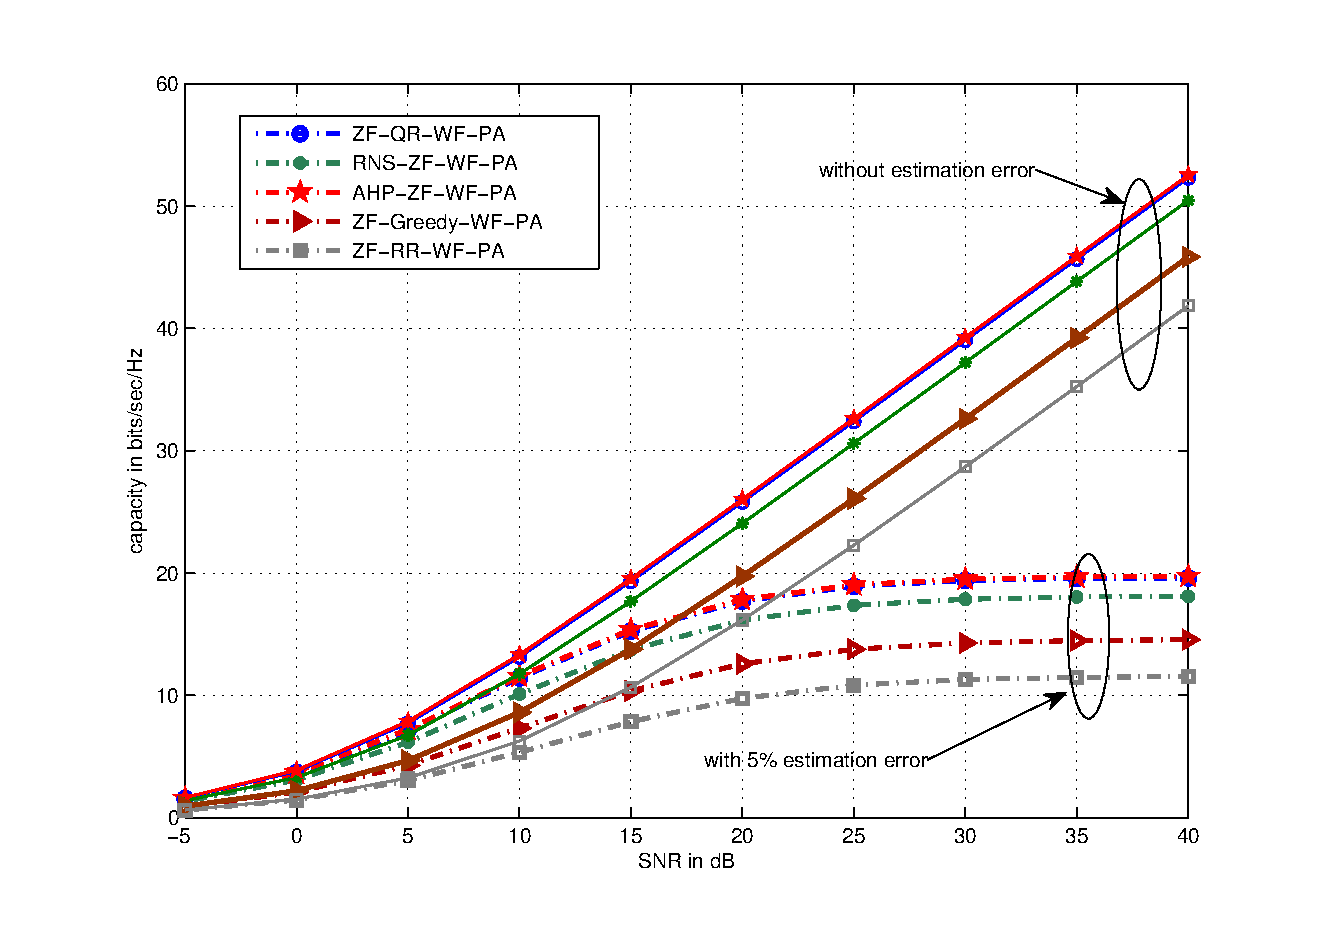
\includegraphics[width=0.8\textwidth]{single-bs-1}
\caption[short]{Sum capacity for \me{\card{\mc{U}} = 20, \, N_\mrm{T} = 4, \, N_\mrm{R} = 1}}
\label{single-bs-f1}
\end{figure}

Fig. \ref{single-bs-f1} compares the performance of capacity achieving user selection schemes discussed in section \ref{mtbus} to the QR based user selection scheme discussed in \cite{antti_user_selection,jin2010novel}. The AHP based user selection provides marginal but still noticeable performance improvement over the existing QR based algorithm. The gain is mainly attributed to the selection mechanism which takes pair-wise channel correlation metric in to account. This additional information is not of great value as it can be seen but the complexity involved in this is significantly large.
\begin{figure}
\centering
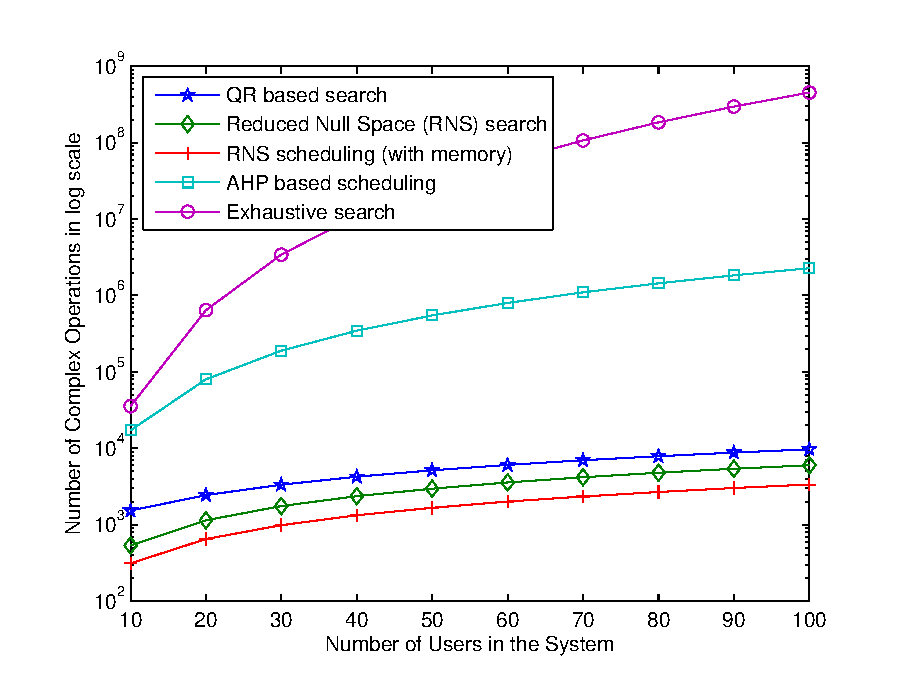
\includegraphics[width=0.8\textwidth]{single-bs-2}
\caption[short]{Scaling of complexity over users for \me{N_\mrm{T} = 4, \, N_\mrm{R} = 1} system}
\label{single-bs-f2}
\end{figure}

Fig. \ref{single-bs-f1} also shows the performance of reduced null space (RNS) scheme which performs closer to the existing QR algorithm but with huge reduction in the complexity involved in the metric calculation. Since QR based schemes requires matrix inverse computation for null space, RNS scheme provides a sub-optimal alternative to achieve the same. Fig. \ref{single-bs-f2} compares the complexity involved in performing various schemes discussed so far. The complexity involved in RNS user selection scheme is the least among the scheduling schemes based on channel correlation discussed here. The complexity can further be reduced by saving the earlier results in the memory (with some increase in the storage memory) to avoid redundant calculations over each iterations. 

The performance of estimation error is also analyzed in Fig. \ref{single-bs-f1} which shows significant degradation over the perfect channel assumption. The estimation error degrades the performance by altering the precoders from being the perfect channel inverse there by creating interference among the transmitted streams. This effect is more pronounced at higher SNR as the capacity is starts saturating since the noise component is dominated by the interference in comparison with the AWGN.


\subsection{Multi BS-US}


This section discusses the user selection schemes discussed in sections \ref{sus} and \ref{cus}. The users are assumed to be located at the cell-edge and the objective is to maximize the achievable capacity of the system. The precoding schemes considered here are based on combined zero-forcing with water-filling (CZF-WF) and W-MMSE based joint precoding and scheduling design discussed in \cite{wmmse_shi}. The W-MMSE scheme performs joint precoding and scheduling of users with the maximizing sum capacity objective. The ZF scheme performs only precoder design for the users in \me{\mc{S}_b} which mandates the users to be selected in way to maximize the sum capacity. The selection of users for multi-BS system needs to be exhaustive in order to achieve the capacity attaining user set \me{\mc{S}_b}. The static user scheduling (SUS) and coordinated user scheduling (CUS) provides one such approach in which users can be selected with minimal complexity in comparison with the exhaustive user search. The user selection schemes discussed earlier provides the better transmission set compared with the conventional user selection scheme for sum rate objective.
\begin{figure}
\centering
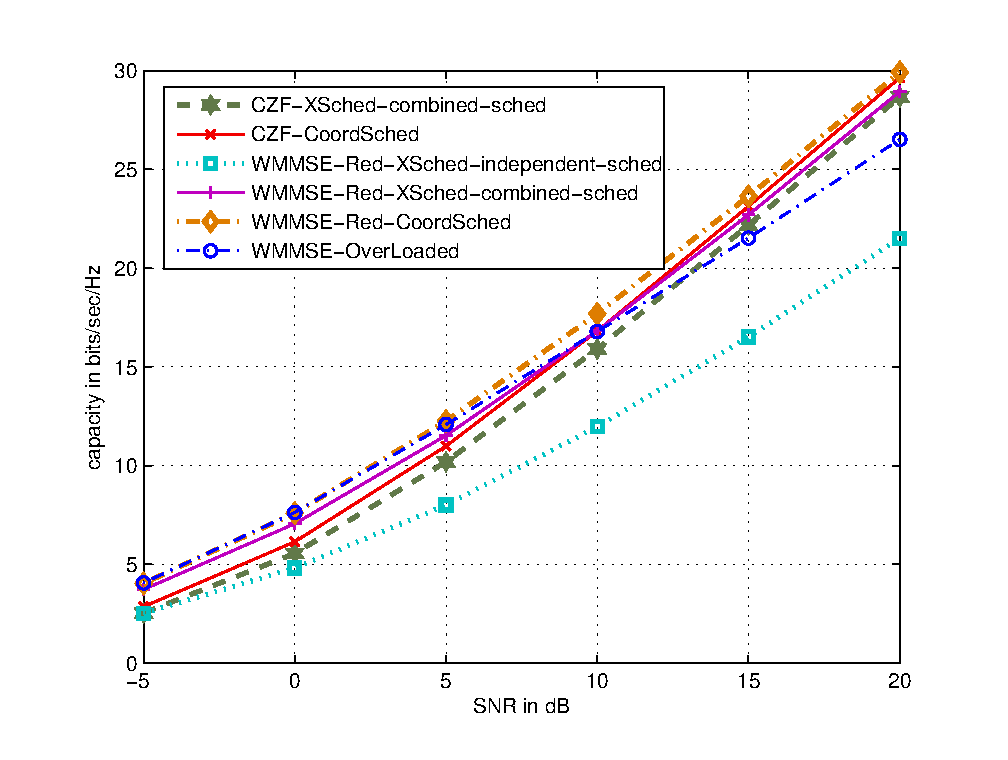
\includegraphics[width=0.8\textwidth]{multi-bs-1}
\caption[short]{Sum capacity for \me{\card{\mc{B}} = 2, \, \card{\mc{U}_k} = 25, \, N_\mrm{T} = 4, \, N_\mrm{R} = 1}}
\label{multi-bs-f1}
\end{figure}

Fig. \ref{multi-bs-f1} shows the comparison of the above mentioned schemes using CZF-WF and W-MMSE precoding designs. The CZF-WF based design is equivalent to W-MMSE scheme at higher SNR when the transmission user set \me{\mc{S}_b} is defined. The reduced W-MMSE scheme is performed over the transmission user set \me{\mc{S}_b \fall b \inm \mc{B}} in contrast with the overloaded W-MMSE scheme performing over the entire user set \me{\mc{U}_b}. The performance of the overloaded W-MMSE scheme degrades as the SNR increases to that of reduced W-MMSE scheme with SUS based user selection for the same stopping resolution \me{\epsilon} as defined in \cite{wmmse_shi}. Even though overloaded W-MMSE performs better at lower SNRs, the reduced W-MMSE using SUS based user selection provides significantly improved performance at higher SNR owing to the fact of reduced variables involved in the optimization problem. The variable reduction is mainly achieved by the selection scheme performed using SUS.

Fig. \ref{multi-bs-f1} plots the performance of CUS scheme as well in comparison with SUS schemes using W-MMSE over reduced user set obtained by the selection algorithms. The CUS scheme provides improved performance by selecting users over the entire user set \me{\mc{U}} for all BSs in \me{\mc{B}} instead selecting over \me{\mc{U}_b} for BS \me{b, \fall b \inm{\mc{B}}}. The CUS scheme avails the additional multi-user selection diversity over conventional SUS based schemes to achieve significant performance improvement. The CUS performance is limited by the number of users available for selection since more users in \me{\mc{U}_b}, more diverse users in the set thereby SUS also enjoys more multi-user diversity performing closer to CUS scheme. To achieve any gain from CUS scheme over SUS scheme, the user set \me{\mc{U}} over which the scheduling is performed should be at the cell-edge thereby availing the instantaneous fading for scheduling users.
\begin{figure}
\centering
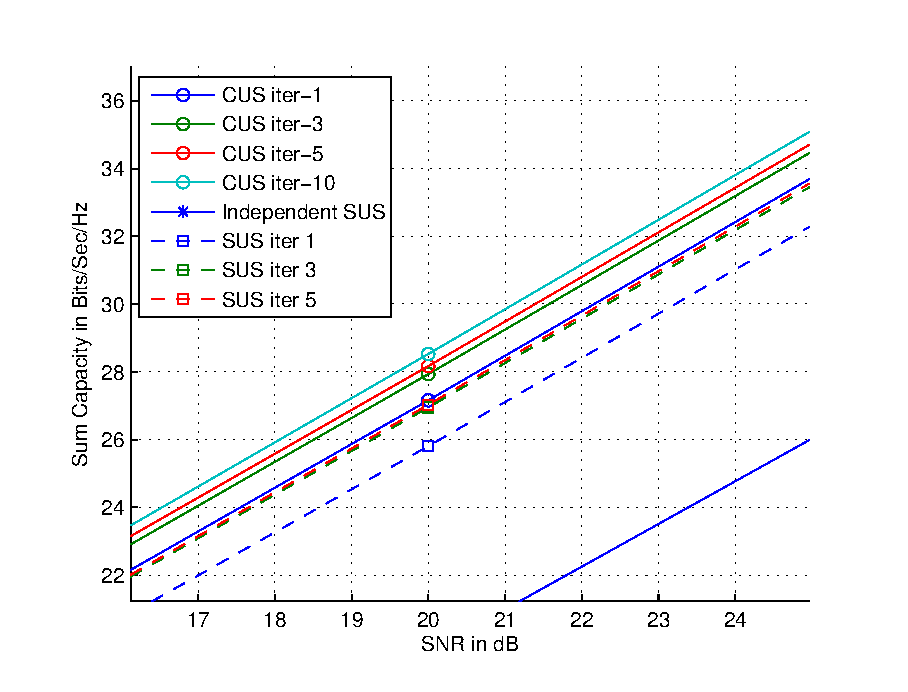
\includegraphics[trim = 0cm 0cm 0cm 7mm, clip, width=0.8\textwidth]{multi-bs-2}
\caption[short]{Iterative sum capacity for \me{\card{\mc{B}} = 2, \, \card{\mc{U}} = 20, \, N_\mrm{T} = 4, \, N_\mrm{R} = 1}}
\label{multi-bs-f2}
\end{figure}

Fig. \ref{multi-bs-f2} depicts the iterative performance improvement of CUS and SUS schemes for different iteration count using sum capacity as the metric. Since the search space is bounded by the user sets \me{\mc{U}, \: \mc{U}_b}, the performance at each iteration will be monotonic in terms of sum rate objective. The selected set at each iterations will be at least good as the earlier transmission user set \me{\mc{S}_b} but not inferior in terms of sum rate metric as shown in Fig. \ref{multi-bs-f2}.


\section{Conclusion}

\bibliographystyle{ieeetr}
\bibliography{./../Library/kirja_survey}

\end{document}
